%=============================================================================
% SECCIÓN DE ANEXOS (ESTRUCTURADA COMO SECCIÓN FORMAL AL IGUAL QUE BIBLIOGRAFÍA)
%=============================================================================

\newpage
\phantomsection
\addcontentsline{toc}{section}{ANEXOS}
\section*{ANEXOS}

\setcounter{figure}{0}
\setcounter{table}{0}
\renewcommand{\thefigure}{A.\arabic{figure}}
\renewcommand{\thetable}{A.\arabic{table}}
\captionsetup{list=no} % Para que no aparezca en índice de figuras del cuerpo preliminar

\subsection*{Anexo 1: Diagrama de bloques funcional de la propuesta de solución mecatrónica}
\label{anx:diagrama_bloques}
\addcontentsline{toc}{subsection}{Anexo 1. Diagrama de bloques funcional de la propuesta de solución}

\begin{figure}[H]
    \centering
    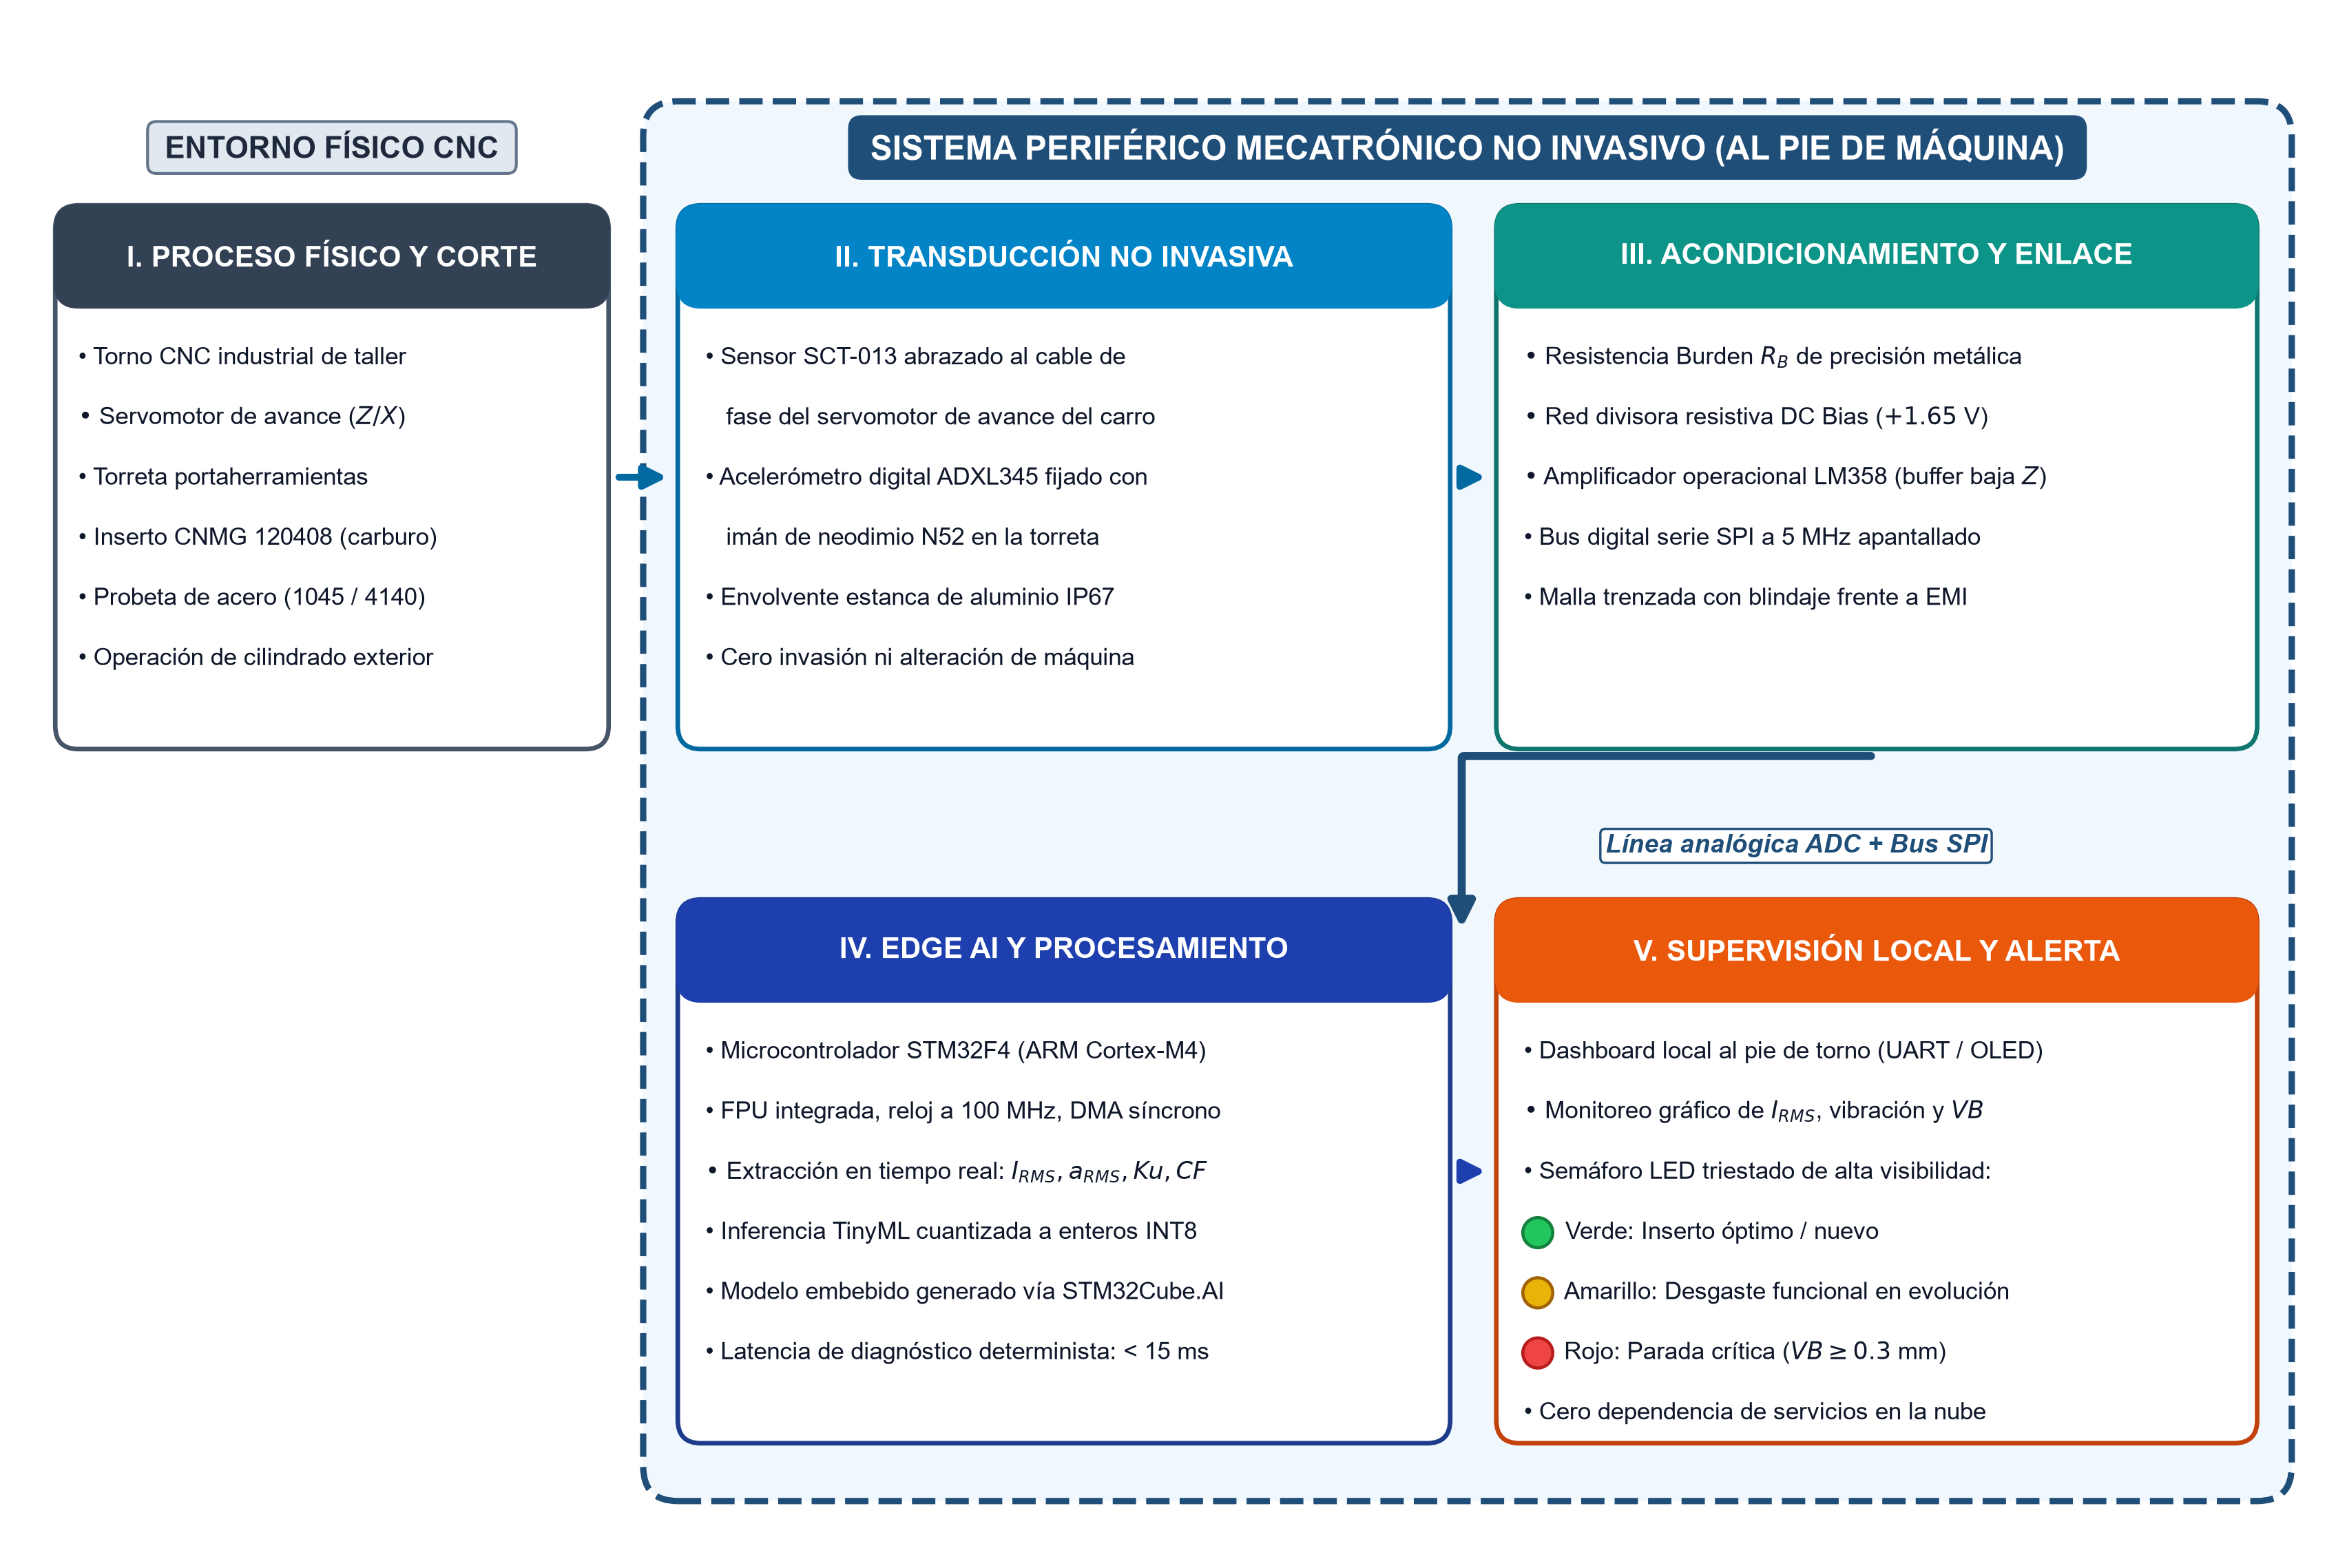
\includegraphics[width=\textwidth]{Figuras/diagrama_bloques_propuesta_solucion.png}
    \caption{Diagrama de bloques funcional general de la arquitectura mecatrónica periférica para monitoreo no invasivo en tornos CNC}
    \vspace{2mm}
    \small \textbf{Fuente:} Elaboración propia, 2026
    \label{fig:anexo_diagrama_bloques}
\end{figure}

El presente anexo describe la arquitectura mecatrónica general y la interconexión modular del sistema periférico propuesto al pie de máquina en taller, estructurado en cinco módulos de ingeniería:

\begin{enumerate}[leftmargin=0.8cm]
    \item \textbf{Módulo I (Entorno Físico CNC y Proceso de Corte):} Corresponde al torno CNC de bancada inclinada y carro móvil en Maestranza San Carlos (MAINSA), donde se ejecutan los ciclos de torneado exterior sobre barras de acero AISI 1045 y 4140 bajo condiciones de refrigeración por taladrina. La interacción de corte sobre el inserto CNMG 120408 transmite esfuerzos hacia el carro longitudinal (eje $Z$) y transversal (eje $X$), así como perturbaciones vibratorias a través de la torreta portaherramientas.
    \item \textbf{Módulo II (Transducción Sensorial No Invasiva):} Disposición periférica del sensor de corriente de núcleo partido SCT-013 abrazado externamente a una de las fases de alimentación del servomotor de avance del carro portaherramientas (eje $Z$) en el armario eléctrico, y del acelerómetro digital triaxial ADXL345 fijado a la torreta mediante base magnética de neodimio N52 en cápsula estanca IP67.
    \item \textbf{Módulo III (Acondicionamiento Analógico y Enlace Digital Industrial):} Red divisora resistiva de polarización DC Bias ($+1.65\,\text{V}$), resistencia Burden de precisión $R_B$, amplificador operacional LM358 configurado como seguidor de tensión de baja impedancia para adecuar la señal al rango del ADC (0 a 3.3~V), y bus digital serie SPI apantallado a 5~MHz con aislamiento frente a interferencia electromagnética (EMI).
    \item \textbf{Módulo IV (Cerebro Mecatrónico y Edge AI):} Unidad de procesamiento embebido sobre microcontrolador STM32F4 (ARM Cortex-M4 @ 100~MHz), con adquisición síncrona por DMA multicanal a 12 bits, filtrado digital Butterworth, ventaneo sincrónico activo durante el arranque de viruta ($I_a > I_{\text{vacío}}$), extracción de descriptores estadísticos temporales y frecuenciales ($I_{\text{RMS}}, a_{\text{RMS}}, Ku, CF$) e inferencia determinista ($<15\,\text{ms}$) con clasificador TinyML cuantizado en enteros de 8 bits (INT8) mediante STM32Cube.AI.
    \item \textbf{Módulo V (Supervisión Local y Alerta Visual en Planta):} Despliegue de métricas en panel gráfico local (dashboard) al pie del torno comunicado vía UART/RS485, e indicación luminosa triestado mediante semáforo LED de alta visibilidad: verde (inserto óptimo), amarillo (desgaste funcional moderado) y rojo (alerta crítica de parada preventiva por desgaste de flanco $VB \ge 0.3\,\text{mm}$ según norma ISO 3685).
\end{enumerate}